\section{Additional material on Section~\ref{sec:application-covid}}\label{sec:appendix-application-covid}


\begin{figure}
    \centering
    \begin{subfigure}[t]{.48\textwidth}
        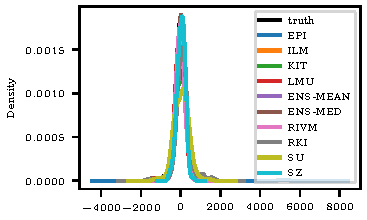
\includegraphics{plots/covid_nowcast/20_kde_lag_1}
        \caption{\ac{kde} for true values and nowcasts of lag 1.}
    \end{subfigure}\hspace{0.01\textwidth}
    \begin{subfigure}[t]{.48\textwidth}
        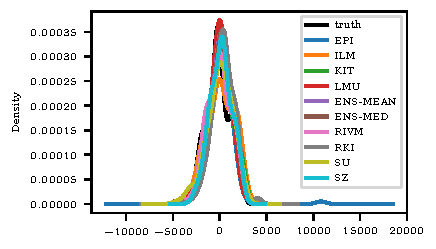
\includegraphics{plots/covid_nowcast/20_kde_lag_7}
        \caption{\ac{kde} for true values and nowcasts of lag 7.}
    \end{subfigure}\hspace{0.01\textwidth}
    \begin{subfigure}[t]{.48\textwidth}
        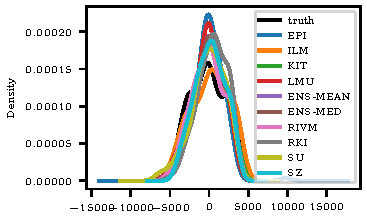
\includegraphics{plots/covid_nowcast/20_kde_lag_14}
        \caption{\ac{kde} for true values and nowcasts of lag 14.}
    \end{subfigure}
    \caption{\Ac{kde} for true values and nowcasts of lags 1, 7, and 14 to assess the distribution of values. \hl{AUSWERTUNG}. Exclusion areas based on the 10\%  quantile of absolute values are listed in Table~\ref{tab:app-covid-marginals}.}
    \label{fig:app-covid-kde}
\end{figure}


\begin{table}
    \centering
    \begin{tabular}{l l}
        \toprule
        Abbreviation & Nowcasting hub key \\
        \midrule
        EPI & Epiforecasts-independent \\
        ILM & ILM-prop \\
        KIT & KIT-simple\_nowcast \\
        LMU & LMU\_StaBLab-GAM\_nowcast \\
        RIVM & RIVM-KEW \\
        RKI & RKI-weekly\_report \\
        SU & SU-hier\_bayes \\
        SZ & SZ-hosp\_nowcast\\
        ENS-MEAN & NowcastHub-MeanEnsemble\\
        ENS-MED & NowcastHub-MedianEnsemble\\
        \bottomrule
    \end{tabular}
    \caption{Matching of the abbreviation to the key in the nowcasting hub. Information on the models and references is listed in \textcite[][Table 1]{Wolffram2023}.}
    \label{tab:app-covid-models}
\end{table}


\begin{table}
    \centering
    \begin{tabularx}{\textwidth}{Xlllllllll}
\toprule
 & (1), l=1 & $\sigma_{x^{\Delta, 1}}$ & $q_{0.1} (x^{\Delta, 1})$ & (1), l=7 & $\sigma_{x^{\Delta, 7}}$ & $q_{0.1} (x^{\Delta, 7})$ & (1), l=14 & $\sigma_{x^{\Delta, 14}}$ & $q_{0.1} (x^{\Delta, 14})$ \\
\midrule
EPI & 86 & 520 & 44 & 83 & 1411 & 78 & 80 & 1976 & 144 \\
ILM & 86 & 281 & 26 & 81 & 1457 & 102 & 82 & 2356 & 140 \\
KIT & 84 & 354 & 50 & 89 & 1306 & 171 & 83 & 1964 & 265 \\
LMU & 65 & 285 & 26 & 84 & 1180 & 124 & 78 & 1946 & 167 \\
ENS-MEAN & 85 & 267 & 23 & 86 & 1213 & 98 & 83 & 1955 & 235 \\
ENS-MED & 88 & 259 & 23 & 88 & 1206 & 101 & 81 & 1955 & 186 \\
RIVM & 77 & 241 & 32 & 81 & 1264 & 123 & 77 & 2034 & 190 \\
RKI & 99 & 362 & 34 & 106 & 1194 & 145 & 99 & 1832 & 325 \\
SU & 91 & 376 & 47 & 85 & 1390 & 180 & 80 & 2126 & 263 \\
SZ & 92 & 201 & 26 & 89 & 1154 & 184 & 87 & 1889 & 241 \\
True & 75 & 262 & 27 & 66 & 1237 & 126 & 73 & 2193 & 284 \\
\bottomrule
\end{tabularx}

    \caption{Analysis of the nowcast and true differences for the lags 1, 7, and 14 days.}
    \label{tab:app-covid-marginals}
\end{table}

\begin{table}
    \centering
    \begin{subfigure}[t]{\textwidth}
        \begin{tabular}{l p{0.11\textwidth} p{0.11\textwidth} p{0.11\textwidth} p{0.11\textwidth} p{0.11\textwidth} p{0.11\textwidth}}
\toprule
 & $\mu^{1}$ & $\mu^{+, 1}$ & $\mu^{-, 1}$ & $\mu^{1}_{q_{0.1}}$ & $\mu^{+, 1}_{q_{0.1}}$ & $\mu^{-, 1}_{q_{0.1}}$ \\
\midrule
EPI & {0.68\newline(0.62, 0.74)} & {0.64\newline(0.55, 0.72)} & {0.73\newline(0.63, 0.81)} & {0.69\newline(0.63, 0.75)} & {0.64\newline(0.56, 0.73)} & {0.75\newline(0.65, 0.82)} \\
ILM & {0.73\newline(0.67, 0.79)} & {0.67\newline(0.58, 0.76)} & {0.82\newline(0.73, 0.89)} & {0.74\newline(0.68, 0.79)} & {0.68\newline(0.60, 0.76)} & {0.82\newline(0.72, 0.89)} \\
KIT & {0.62\newline(0.55, 0.68)} & {0.58\newline(0.49, 0.67)} & {0.65\newline(0.56, 0.75)} & {0.62\newline(0.56, 0.69)} & {0.59\newline(0.51, 0.67)} & {0.66\newline(0.57, 0.74)} \\
LMU & {0.66\newline(0.60, 0.72)} & {0.66\newline(0.57, 0.75)} & {0.66\newline(0.57, 0.73)} & {0.66\newline(0.59, 0.72)} & {0.66\newline(0.55, 0.75)} & {0.66\newline(0.57, 0.73)} \\
ENS-MEAN & {0.81\newline(0.75, 0.85)} & {0.76\newline(0.68, 0.84)} & {0.88\newline(0.81, 0.93)} & {0.81\newline(0.75, 0.86)} & {0.76\newline(0.68, 0.83)} & {0.88\newline(0.81, 0.94)} \\
ENS-MED & {0.75\newline(0.68, 0.80)} & {0.69\newline(0.60, 0.77)} & {0.81\newline(0.73, 0.89)} & {0.75\newline(0.69, 0.80)} & {0.69\newline(0.61, 0.77)} & {0.83\newline(0.74, 0.90)} \\
RIVM & {0.77\newline(0.72, 0.82)} & {0.75\newline(0.66, 0.83)} & {0.79\newline(0.71, 0.85)} & {0.78\newline(0.72, 0.83)} & {0.75\newline(0.66, 0.83)} & {0.81\newline(0.73, 0.87)} \\
RKI & {0.74\newline(0.68, 0.80)} & {0.67\newline(0.59, 0.75)} & {0.88\newline(0.79, 0.93)} & {0.74\newline(0.67, 0.79)} & {0.66\newline(0.58, 0.73)} & {0.87\newline(0.78, 0.93)} \\
SU & {0.71\newline(0.65, 0.77)} & {0.66\newline(0.57, 0.74)} & {0.78\newline(0.69, 0.85)} & {0.72\newline(0.66, 0.78)} & {0.67\newline(0.58, 0.75)} & {0.79\newline(0.70, 0.87)} \\
SZ & {0.74\newline(0.69, 0.80)} & {0.68\newline(0.60, 0.76)} & {0.82\newline(0.73, 0.88)} & {0.74\newline(0.69, 0.80)} & {0.68\newline(0.60, 0.76)} & {0.82\newline(0.73, 0.88)} \\
\bottomrule
\end{tabular}

    \caption{1 day.}
    \end{subfigure}
    \begin{subfigure}[t]{\textwidth}
        \begin{tabular}{l p{0.11\textwidth} p{0.11\textwidth} p{0.11\textwidth} p{0.11\textwidth} p{0.11\textwidth} p{0.11\textwidth}}
\toprule
 & $\mu^{1}$ & $\mu^{+, 1}$ & $\mu^{-, 1}$ & $\mu^{1}_{q_{0.1}}$ & $\mu^{+, 1}_{q_{0.1}}$ & $\mu^{-, 1}_{q_{0.1}}$ \\
\midrule
EPI & {0.68\newline(0.62, 0.74)} & {0.64\newline(0.55, 0.72)} & {0.73\newline(0.63, 0.81)} & {0.69\newline(0.63, 0.75)} & {0.64\newline(0.56, 0.73)} & {0.75\newline(0.65, 0.82)} \\
ILM & {0.73\newline(0.67, 0.79)} & {0.67\newline(0.58, 0.76)} & {0.82\newline(0.73, 0.89)} & {0.74\newline(0.68, 0.79)} & {0.68\newline(0.60, 0.76)} & {0.82\newline(0.72, 0.89)} \\
KIT & {0.62\newline(0.55, 0.68)} & {0.58\newline(0.49, 0.67)} & {0.65\newline(0.56, 0.75)} & {0.62\newline(0.56, 0.69)} & {0.59\newline(0.51, 0.67)} & {0.66\newline(0.57, 0.74)} \\
LMU & {0.66\newline(0.60, 0.72)} & {0.66\newline(0.57, 0.75)} & {0.66\newline(0.57, 0.73)} & {0.66\newline(0.59, 0.72)} & {0.66\newline(0.55, 0.75)} & {0.66\newline(0.57, 0.73)} \\
ENS-MEAN & {0.81\newline(0.75, 0.85)} & {0.76\newline(0.68, 0.84)} & {0.88\newline(0.81, 0.93)} & {0.81\newline(0.75, 0.86)} & {0.76\newline(0.68, 0.83)} & {0.88\newline(0.81, 0.94)} \\
ENS-MED & {0.75\newline(0.68, 0.80)} & {0.69\newline(0.60, 0.77)} & {0.81\newline(0.73, 0.89)} & {0.75\newline(0.69, 0.80)} & {0.69\newline(0.61, 0.77)} & {0.83\newline(0.74, 0.90)} \\
RIVM & {0.77\newline(0.72, 0.82)} & {0.75\newline(0.66, 0.83)} & {0.79\newline(0.71, 0.85)} & {0.78\newline(0.72, 0.83)} & {0.75\newline(0.66, 0.83)} & {0.81\newline(0.73, 0.87)} \\
RKI & {0.74\newline(0.68, 0.80)} & {0.67\newline(0.59, 0.75)} & {0.88\newline(0.79, 0.93)} & {0.74\newline(0.67, 0.79)} & {0.66\newline(0.58, 0.73)} & {0.87\newline(0.78, 0.93)} \\
SU & {0.71\newline(0.65, 0.77)} & {0.66\newline(0.57, 0.74)} & {0.78\newline(0.69, 0.85)} & {0.72\newline(0.66, 0.78)} & {0.67\newline(0.58, 0.75)} & {0.79\newline(0.70, 0.87)} \\
SZ & {0.74\newline(0.69, 0.80)} & {0.68\newline(0.60, 0.76)} & {0.82\newline(0.73, 0.88)} & {0.74\newline(0.69, 0.80)} & {0.68\newline(0.60, 0.76)} & {0.82\newline(0.73, 0.88)} \\
\bottomrule
\end{tabular}

        \caption{14 days.}
    \end{subfigure}
    \caption{Trending ratio $\acc$, positive trending ratio $\accp$, and negative trending ratio $\accm$ for the models with and without exclusion areas for the lag 1 and 14 days. The exclusion areas are rectangles centered on the zero points with width and height of 10\% of the quantile of the absolute values of nowcast and true values. }
    \label{tab:app-covid-trending-ratios-lag-1-14}
\end{table}



\begin{figure}
\centering
\begin{subfigure}[t]{0.23\textwidth}
    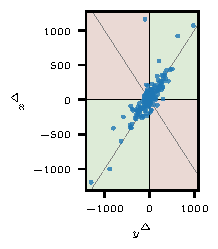
\includegraphics{plots/covid_nowcast/30_ENS-MEAN_4q_lag_1}
    \caption{ENS-Mean, lag 1 day}\label{fig:app-covid-4q-ens-mean-1}
\end{subfigure}\hspace{0.01\textwidth}%
\begin{subfigure}[t]{0.23\textwidth}
    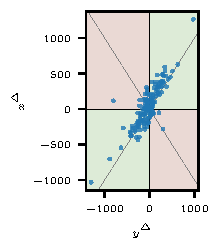
\includegraphics{plots/covid_nowcast/30_ILM_4q_lag_1}
    \caption{ILM, lag 1 day}\label{fig:app-covid-4q-ilm-1}
\end{subfigure}\hspace{0.01\textwidth}%
\begin{subfigure}[t]{0.23\textwidth}
    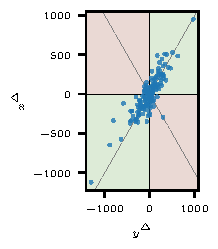
\includegraphics{plots/covid_nowcast/30_RIVM_4q_lag_1}
    \caption{RIVM, lag 1 day}\label{fig:app-covid-4q-rivm-1}
\end{subfigure}\hspace{0.01\textwidth}%
\begin{subfigure}[t]{0.23\textwidth}
    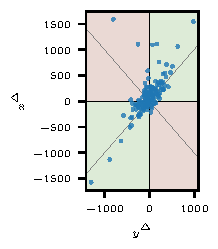
\includegraphics{plots/covid_nowcast/30_RKI_4q_lag_1}
    \caption{RKI, lag 1 day}\label{fig:app-covid-4q-rki-1}
\end{subfigure}
% lag 7
\begin{subfigure}[t]{0.23\textwidth}
    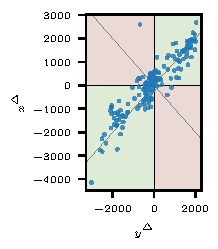
\includegraphics{plots/covid_nowcast/30_ENS-MEAN_4q_lag_7}
    \caption{ENS-Mean, lag 7 days}\label{fig:app-covid-4q-ens-mean-7}
\end{subfigure}\hspace{0.01\textwidth}%
\begin{subfigure}[t]{0.23\textwidth}
    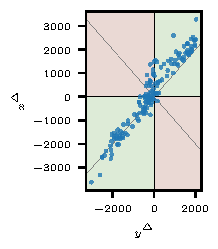
\includegraphics{plots/covid_nowcast/30_ILM_4q_lag_7}
    \caption{ILM, lag 7 days}\label{fig:app-covid-4q-ilm-7}
\end{subfigure}\hspace{0.01\textwidth}%
\begin{subfigure}[t]{0.23\textwidth}
    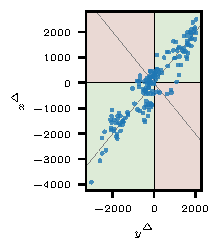
\includegraphics{plots/covid_nowcast/30_RIVM_4q_lag_7}
    \caption{RIVM, lag 7 days}\label{fig:app-covid-4q-rivm-7}
\end{subfigure}\hspace{0.01\textwidth}%
\begin{subfigure}[t]{0.23\textwidth}
    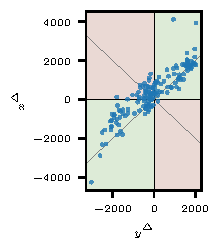
\includegraphics{plots/covid_nowcast/30_RKI_4q_lag_7}
    \caption{RKI, lag 7 days}\label{fig:app-covid-4q-rki-7}
\end{subfigure}
% lag 14
\begin{subfigure}[t]{0.23\textwidth}%
    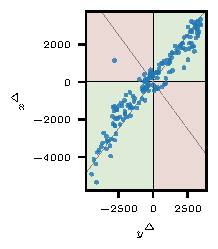
\includegraphics{plots/covid_nowcast/30_ENS-MEAN_4q_lag_14}
    \caption{ENS-Mean, lag 14 days}\label{fig:app-covid-4q-ens-mean-14}
\end{subfigure}\hspace{0.01\textwidth}
\begin{subfigure}[t]{0.23\textwidth}%
    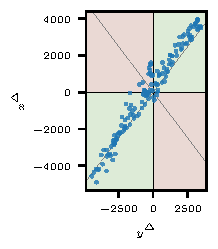
\includegraphics{plots/covid_nowcast/30_ILM_4q_lag_14}
    \caption{ILM, lag 14 days}\label{fig:app-covid-4q-ilm-14}
\end{subfigure}\hspace{0.01\textwidth}
\begin{subfigure}[t]{0.23\textwidth}%
    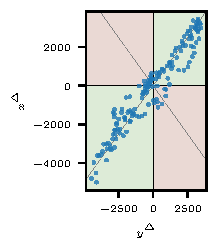
\includegraphics{plots/covid_nowcast/30_RIVM_4q_lag_14}
    \caption{RIVM, lag 14 days}\label{fig:app-covid-4q-rivm-14}
\end{subfigure}\hspace{0.01\textwidth}%
\begin{subfigure}[t]{0.23\textwidth}
    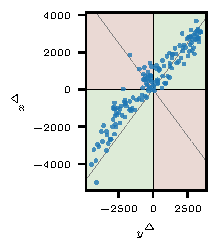
\includegraphics{plots/covid_nowcast/30_RKI_4q_lag_14}
    \caption{RKI, lag 14 days}\label{fig:app-covid-4q-rki-14}
\end{subfigure}%
\caption{Four-quadrant plots for the models ILM, RIVM, RKI, and ENS-MEAN and the lags of one, seven, and 14 days. }
\label{fig:app-covid-4q}
\end{figure}
